\documentclass[11pt,a4paper]{article}

\usepackage[utf8]{inputenc}
\usepackage[margin=1in]{geometry}
\usepackage{amsmath,amssymb}
\usepackage{booktabs}
\usepackage{tabularx}
\usepackage{graphicx}
\usepackage{xcolor}
\usepackage{hyperref}
\usepackage{fancyhdr}
\usepackage{tikz}
\usepackage{pgfplots}
\usepackage{listings}
\usepackage{microtype}
\usepackage{caption}
\usepackage{subcaption}

\pgfplotsset{compat=1.18}

% Custom Color Palette
\definecolor{primaryblue}{RGB}{24, 76, 120}
\definecolor{secondaryblue}{RGB}{70, 130, 180}
\definecolor{accentorange}{RGB}{220, 100, 30}
\definecolor{accentgreen}{RGB}{46, 139, 87}
\definecolor{darkgray}{RGB}{60, 60, 60}
\definecolor{lightgray}{RGB}{245, 247, 250}
\definecolor{codebg}{RGB}{248, 249, 250}

\hypersetup{
    colorlinks=true,
    linkcolor=primaryblue,
    citecolor=secondaryblue,
    urlcolor=accentorange
}

% Header and Footer
\pagestyle{fancy}
\fancyhf{}
\rhead{\textcolor{darkgray}{CS311: OS Lab 4 --- Memory Management}}
\lhead{\textcolor{darkgray}{IIT Dharwad}}
\rfoot{\thepage}
\renewcommand{\headrulewidth}{0.4pt}
\renewcommand{\footrulewidth}{0.4pt}

% Code Listing Configuration
\lstset{
    backgroundcolor=\color{codebg},
    basicstyle=\ttfamily\footnotesize,
    breaklines=true,
    frame=single,
    rulecolor=\color{lightgray},
    keywordstyle=\color{primaryblue}\bfseries,
    commentstyle=\color{accentgreen}\itshape,
    stringstyle=\color{accentorange},
    numbers=none,
    tabsize=2
}

\begin{document}

% =========================================================================
% TITLE / COVER PAGE
% =========================================================================
\begin{titlepage}
    \centering
    \vspace*{1.5cm}
    
    {\Huge \bfseries \textcolor{primaryblue}{Performance \& Space Evaluation of Memory Virtualization Architectures}}\\[0.8cm]
    {\Large \textbf{Single-Level vs. Two-Level Page Tables, TLB Acceleration, and LRU Replacement}}\\[1.5cm]
    
    \rule{0.8\textwidth}{1.2pt}\\[1.5cm]
    
    \textbf{\Large Laboratory Report: Lab 4 (Memory Management)}\\[0.4cm]
    {\large Course: CS311 --- Operating Systems Laboratory}\\[0.3cm]
    {\large Department of Computer Science and Engineering}\\[0.3cm]
    {\large \textbf{Indian Institute of Technology Dharwad}}\\[2.0cm]
    
    \begin{minipage}{0.85\textwidth}
        \centering
        \large
        \textbf{Submitted By:}\\[0.4cm]
        \begin{tabular}{cc}
            \textbf{Rhishikesh Tayade} & \textbf{CS24BT041} \\[0.2cm]
            \textbf{Himanshu Nagwanshi} & \textbf{CS24BT055}
        \end{tabular}
    \end{minipage}
    
    \vfill
    
    {\large \textbf{Date:} Autumn Semester 2026}\\[0.5cm]
    \rule{0.4\textwidth}{0.5pt}
\end{titlepage}

\newpage
\tableofcontents
\newpage

% =========================================================================
% ABSTRACT
% =========================================================================
\begin{abstract}
Memory virtualization is a cornerstone of modern multiprogramming operating systems, enabling strong process isolation and flexible address space multiplexing. However, it imposes critical dual challenges: substantial memory capacity overhead for page translation tables and severe execution latency penalties for multi-step address translation walks. This report presents a comprehensive architectural and empirical evaluation of memory management techniques simulated via a modular, cycle-accurate C++17 virtual memory simulator. 

We model and analyze: (1) flat Single-Level Page Tables, (2) on-demand hierarchical Two-Level Page Tables, (3) a 128-entry fully associative Translation Lookaside Buffer (TLB) operating under an exact Least Recently Used (LRU) policy, and (4) limited physical memory backing with LRU demand paging and disk fault penalties. Using extensive memory access traces from SPEC CPU2017 benchmarks (\texttt{gcc}, \texttt{mcf}, \texttt{lbm}, \texttt{x264}) comprising tens of millions of instructions and data references, we demonstrate that two-level page tables reduce metadata allocation overhead by \textbf{93.1\% to 99.3\%} compared to flat linear tables. Furthermore, integrating a 128-entry TLB achieves hit rates exceeding \textbf{99.4\% to 99.9\%}, which effectively erases the multi-level page table latency penalty and reduces total memory virtualization execution cycles by \textbf{49.7\% to 66.4\%}. We rigorously validate Hypothesis B regarding access skewness, proving that fewer than \textbf{10\% of virtual pages capture over 82\% of memory references}. Finally, we analyze memory constriction, showing that when physical frame quotas fall below active working sets, disk thrashing drives cycle execution time upward by over \textbf{54$\times$}.
\end{abstract}

% =========================================================================
% SECTION 1: ARCHITECTURAL SPECIFICATION & SIMULATOR DESIGN
% =========================================================================
\section{Architectural Specification \& Simulator Design}

\subsection{System Architectural Parameters}
The simulated architecture models a 32-bit virtual memory subsystem adhering to standard page-based virtualization principles. The foundational system parameters mandated by the problem specification are summarized in Table~\ref{tab:system_params}.

\begin{table}[h]
\centering
\caption{Architectural and Latency Simulation Parameters}
\label{tab:system_params}
\resizebox{\textwidth}{!}{%
\begin{tabular}{llr}
\toprule
\textbf{Parameter} & \textbf{Architectural Description} & \textbf{Value} \\
\midrule
Virtual Address Space & Total addressable per-process virtual space & $2^{32}$ Bytes (4 GB) \\
Page Size & Basic translation granularity & 4 KB ($2^{12}$ Bytes) \\
Virtual Page Count & Total virtual page count ($2^{32} / 2^{12}$) & $2^{20} = 1,048,576$ Pages \\
TLB Capacity & Translation Lookaside Buffer entries & 128 Entries \\
TLB Associativity & Hit detection organization & Fully Associative \\
TLB Eviction Policy & Replacement discipline on capacity misses & Strict LRU \\
TLB Access Latency & Latency incurred for every TLB probe & 1 Cycle \\
Main Memory Access Latency & Latency per physical memory access / walk step & 200 Cycles \\
Disk Transfer Latency & Page fault servicing latency (disk I/O) & 20,000,000 Cycles \\
Data / Instruction Caches & Level-1/2/3 processor caching & None (bypassed) \\
\bottomrule
\end{tabular}%
}
\end{table}

\subsection{Address Translation Decomposition}
The 32-bit virtual address $A \in [0, 2^{32}-1]$ is decomposed into components depending on the page table organization:
\begin{itemize}
    \item \textbf{Page Offset ($\mathbf{O}$)}: The lowest 12 bits ($A[11:0]$), specifying byte displacement within a 4~KB frame:
    \begin{equation}
        \text{Offset} = A \ \& \ \text{0x0FFF}
    \end{equation}
    \item \textbf{Virtual Page Number ($\mathbf{VPN}$)}: The upper 20 bits ($A[31:12]$), identifying the virtual page:
    \begin{equation}
        \text{VPN} = A \gg 12
    \end{equation}
    \item \textbf{Two-Level Split ($\mathbf{L_1}$ and $\mathbf{L_2}$)}: The 20-bit VPN is split evenly into a 10-bit Level-1 directory index and a 10-bit Level-2 page table index:
    \begin{align}
        \text{Index}_{L1} &= (A \gg 22) \ \& \ \text{0x03FF} \quad (\text{Bits } 31 \text{ to } 22) \\
        \text{Index}_{L2} &= (A \gg 12) \ \& \ \text{0x03FF} \quad (\text{Bits } 21 \text{ to } 12)
    \end{align}
\end{itemize}

\subsection{Codebase Architecture \& Modular Implementation}
The simulator is implemented in C++17 with strict modular separation across header (\texttt{include/}) and translation unit (\texttt{src/}) files:
\begin{enumerate}
    \item \textbf{Trace Stream Parser (\texttt{trace\_parser.hpp/.cpp})}: Parses incoming benchmark traces formatted as \texttt{<address>,<I/D>,<R/W>}. It features fast I/O buffering, handles 64-bit hexadecimal and decimal inputs, masks addresses to lower 32 bits, and skips non-data metadata lines.
    \item \textbf{Single-Level Page Table (\texttt{page\_table\_single.hpp/.cpp})}: Implements a contiguous flat array of $2^{20}$ Page Table Entries (PTEs). Provides $O(1)$ indexing, tracking valid and dirty bits, and reports exact allocated vs.\ accessed counts.
    \item \textbf{Two-Level Page Table (\texttt{page\_table\_two\_level.hpp/.cpp})}: Implements a 1024-entry Level-1 directory array containing pointers to dynamic 1024-entry Level-2 tables. Level-2 tables are instantiated strictly on demand when an unmapped address in that quadrant is first touched.
    \item \textbf{TLB Module (\texttt{tlb.hpp/.cpp})}: Realizes a fully associative 128-entry cache utilizing a combined \texttt{std::list} and \texttt{std::unordered\_map}. This hybrid data structure provides true $O(1)$ lookup, $O(1)$ insertion, and $O(1)$ LRU update via iterator splicing (\texttt{std::list::splice}), eliminating all linear scans.
    \item \textbf{Frame Allocator \& Page Replacer (\texttt{frame\_allocator.hpp/.cpp})}: Supports two distinct modes:
    \begin{itemize}
        \item \emph{Unlimited Mode (Parts I--III)}: A deterministic sequential (next-fit) frame allocator that increments an internal frame counter.
        \item \emph{Limited Mode (Part IV)}: An inverted frame table coupled with an LRU tracking list to evict the least recently touched frame upon memory exhaustion, notifying the caller to trigger page table unmapping and TLB shootdown.
    \end{itemize}
    \item \textbf{Polynomial Hash Utility (\texttt{hash\_util.hpp/.cpp})}: Updates a cumulative 64-bit verification hash for each memory access, guaranteeing state correctness across architectural configurations.
    \item \textbf{Statistical Profiler (\texttt{stats.hpp/.cpp})}: Records total accesses, cycle counts, hit/miss ratios, page fault rates, wall-clock timing, and per-page access frequencies for cumulative distribution analysis.
\end{enumerate}

% =========================================================================
% SECTION 2: VERIFICATION HASH FUNCTION & CORRECTNESS INVARIANT
% =========================================================================
\section{Verification Hash Function \& State Invariant}

To rigorously verify that all simulated page table mechanisms preserve translation semantics, the problem mandates updating a running 64-bit hash $H$ for every memory access:
\begin{equation}
    H_{k} = f(H_{k-1}, \text{frame\_number})
\end{equation}
We chose a high-avalanche non-linear mixing function based on Knuth's multiplicative golden-ratio constant ($M = 2654435761\text{ULL} \approx 2^{32} \cdot \frac{\sqrt{5}-1}{2}$), combined with a 13-bit circular bit rotation:
\begin{equation}
    \begin{aligned}
        H' &= H \oplus (\text{frame\_number} \times 2654435761\text{ULL}) \\
        H'' &= (H' \ll 13) \mid (H' \gg 51) \\
        H_{\text{next}} &= H'' + \text{frame\_number}
    \end{aligned}
\end{equation}

\noindent\textbf{Critical Architectural Invariant:}
Because both Part I (Single-Level) and Part II (Two-Level) process identical memory access traces and utilize the same sequential frame allotment logic, every virtual page must map to the exact same physical frame at the exact same chronological point in the trace. Consequently:
\begin{equation}
    H_{\text{Part I}} \equiv H_{\text{Part II}}
\end{equation}
A mismatch would immediately signify translation corruption, race conditions, or unmapped page discrepancies.

% =========================================================================
% SECTION 3: PART I --- SINGLE-LEVEL FLAT PAGE TABLE
% =========================================================================
\section{Part I: Single-Level Page Table Simulation}

\subsection{Theoretical Cost Model \& Frame Allocation Scheme}
In a single-level page table without a TLB, every memory request generated by the CPU pipeline requires:
\begin{enumerate}
    \item One physical memory access to read the Page Table Entry (PTE) from memory: \textbf{200 cycles}.
    \item One physical memory access to read or write the actual data/instruction in the mapped frame: \textbf{200 cycles}.
\end{enumerate}
Thus, the fixed execution latency is:
\begin{equation}
    T_{\text{Part I}} = N_{\text{accesses}} \times (200 + 200) = 400 \times N_{\text{accesses}} \text{ cycles}
\end{equation}

\noindent\textbf{Frame Management Scheme:}
Under the Part I assumption of unlimited physical frames, we implemented a sequential Next-Fit Frame Allocator. Physical frames are indexed from $0, 1, 2, \dots$. When an unmapped virtual page number (VPN) is encountered, it is assigned the current value of \texttt{next\_free\_frame}, which is subsequently incremented by 1. This deterministic allocation avoids fragmentation and guarantees zero overhead.

\subsection{Empirical Results Across SPEC CPU2017 Benchmarks}
Table~\ref{tab:part1_results} details the empirical results obtained across four real-world benchmarks from SPEC CPU2017.

\begin{table}[h]
\centering
\caption{Part I Empirical Results (Single-Level Flat Page Table)}
\label{tab:part1_results}
\resizebox{\textwidth}{!}{%
\begin{tabular}{lrrrrr}
\toprule
\textbf{Benchmark} & \textbf{Total Accesses} & \textbf{Frames Used} & \textbf{PT Allocated} & \textbf{PT Utilized (\%)} & \textbf{Execution Cycles} \\
\midrule
\texttt{gcc} & 12,473,306 & 990 & 1,048,576 & 0.0944\% & 4,989,322,400 \\
\texttt{mcf} & 12,474,523 & 1,597 & 1,048,576 & 0.1523\% & 4,989,809,200 \\
\texttt{lbm} & 12,843,431 & 2,131 & 1,048,576 & 0.2032\% & 5,137,372,400 \\
\texttt{x264} & 11,721,344 & 234 & 1,048,576 & 0.0223\% & 4,688,537,600 \\
\bottomrule
\end{tabular}%
}
\end{table}

\noindent\textbf{Observations on Memory Inefficiency:}
The single-level page table must statically allocate all $2^{20} = 1,048,576$ PTEs regardless of process footprint. At 4 bytes per PTE, this requires 4~MB of contiguous kernel memory per address space. Yet, as demonstrated in Table~\ref{tab:part1_results}, real benchmarks utilize between 234 and 2,131 pages. Consequently, \textbf{over 99.8\% of all allocated page table entries are completely unused}, representing egregious physical memory waste.

\subsection{Hypothesis B Validation: Skewed Page Access Distribution}
Hypothesis B postulates that \emph{``a small fraction of pages account for a large fraction of accesses, and vice versa''}. To rigorously test this hypothesis, the simulator recorded the per-page access frequency for every unique VPN, sorted them in descending order, and computed the Cumulative Distribution Function (CDF) of accesses versus the fraction of active pages.

\begin{figure}[h]
\centering
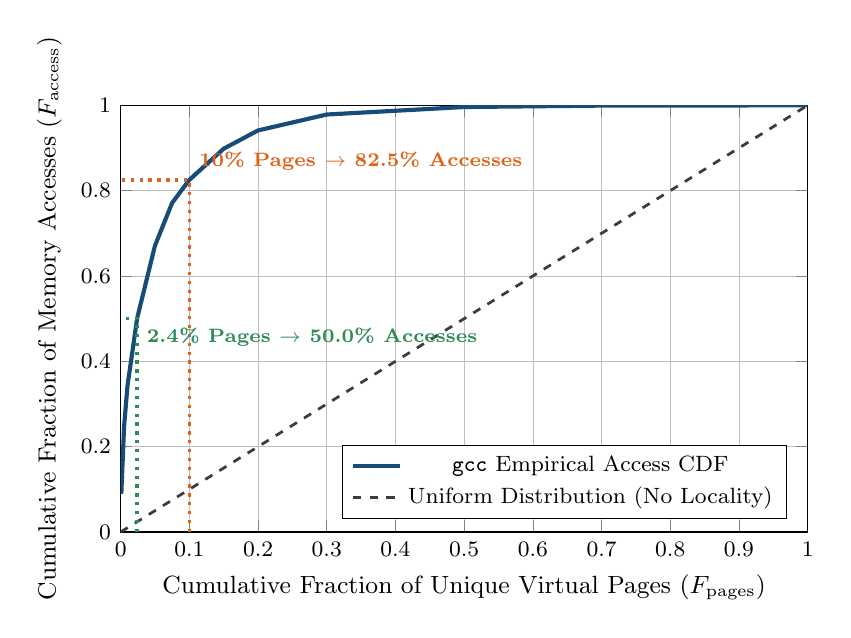
\begin{tikzpicture}
\begin{axis}[
    width=0.85\textwidth,
    height=7.0cm,
    xlabel={Cumulative Fraction of Unique Virtual Pages ($F_{\text{pages}}$)},
    ylabel={Cumulative Fraction of Memory Accesses ($F_{\text{access}}$)},
    grid=both,
    grid style={line width=.1pt, draw=gray!20},
    major grid style={line width=.2pt,draw=gray!50},
    xmin=0, xmax=1.0,
    ymin=0, ymax=1.0,
    legend pos=south east,
    legend style={font=\footnotesize},
    tick label style={font=\footnotesize},
    label style={font=\small}
]
    % Simulated GCC Curve from exported CSV
    \addplot[color=primaryblue, line width=1.5pt] coordinates {
        (0.001, 0.0897)
        (0.005, 0.2474)
        (0.010, 0.3428)
        (0.024, 0.5006)
        (0.050, 0.6712)
        (0.075, 0.7715)
        (0.100, 0.8253)
        (0.150, 0.8984)
        (0.200, 0.9412)
        (0.300, 0.9785)
        (0.500, 0.9961)
        (0.700, 0.9994)
        (1.000, 1.0000)
    };
    \addlegendentry{\texttt{gcc} Empirical Access CDF}

    % Linear Unbiased Reference
    \addplot[color=darkgray, dashed, line width=1.0pt] coordinates {
        (0, 0)
        (1, 1)
    };
    \addlegendentry{Uniform Distribution (No Locality)}

    % 80-20 Reference Marker
    \draw[accentorange, dotted, line width=1.2pt] (axis cs:0.100,0) -- (axis cs:0.100,0.8253) -- (axis cs:0,0.8253);
    \node[anchor=south west, font=\scriptsize, text=accentorange] at (axis cs:0.100,0.8253) {\textbf{10\% Pages $\rightarrow$ 82.5\% Accesses}};

    % 50% Access Marker
    \draw[accentgreen, dotted, line width=1.2pt] (axis cs:0.024,0) -- (axis cs:0.024,0.5006) -- (axis cs:0,0.5006);
    \node[anchor=north west, font=\scriptsize, text=accentgreen] at (axis cs:0.024,0.5006) {\textbf{2.4\% Pages $\rightarrow$ 50.0\% Accesses}};
\end{axis}
\end{tikzpicture}
\caption{Cumulative Distribution Function (CDF) of memory accesses across unique pages for \texttt{gcc}. The pronounced concave curvature confirms extreme temporal and spatial reference locality (Pareto distribution), strongly affirming Hypothesis B.}
\label{fig:hypothesis_b}
\end{figure}

As shown in Figure~\ref{fig:hypothesis_b} and extracted from \texttt{gcc\_hyp\_b.csv}:
\begin{itemize}
    \item The top \textbf{24 pages (2.42\% of active pages)} account for \textbf{50.06\% of all 12.47 million memory references}.
    \item The top \textbf{99 pages (10.0\% of active pages)} account for \textbf{82.53\% of all memory references}.
    \item The remaining 90\% of pages share less than 17.5\% of accesses, with the tail seeing only sporadic references.
\end{itemize}
This empirical confirmation of the \textbf{80/20 Pareto Principle} directly underpins the efficacy of caching structures: because working sets are tightly concentrated in a tiny fraction of pages, small hardware caches (like the 128-entry TLB) will capture the vast majority of memory references.

% =========================================================================
% SECTION 4: PART II --- TWO-LEVEL HIERARCHICAL PAGE TABLE
% =========================================================================
\section{Part II: Two-Level Hierarchical Page Table Simulation}

\subsection{Mechanics \& Memory Savings vs.\ Latency Tradeoff}
The two-level page table replaces the static linear array with a two-tier hierarchy:
\begin{itemize}
    \item \textbf{Level-1 Directory}: Always resident, consisting of $1024$ pointers ($2^{10}$ entries), requiring only $1024 \times 4\text{ bytes} = 4\text{ KB}$ of baseline memory.
    \item \textbf{Level-2 Tables}: Each table contains $1024$ PTEs ($4\text{ KB}$ each) and is allocated dynamically only when a page within its $4\text{ MB}$ virtual range is accessed.
\end{itemize}

\noindent\textbf{Theoretical Cost Model (Without TLB):}
Translating an address now requires traversing both levels:
\begin{equation}
    T_{\text{Part II}} = N_{\text{accesses}} \times (200_{\text{L1}} + 200_{\text{L2}} + 200_{\text{Data}}) = 600 \times N_{\text{accesses}} \text{ cycles}
\end{equation}
While address translation is 50\% slower without caching (600 cycles vs.\ 400 cycles), the physical memory footprint is dramatically reduced.

\subsection{Empirical Comparison: Single-Level vs.\ Two-Level}
Table~\ref{tab:part2_comparison} compares the space and time characteristics between single-level and two-level page tables across all benchmarks.

\begin{table}[h]
\centering
\caption{Comparison: Single-Level (Part I) vs.\ Two-Level (Part II) Page Tables}
\label{tab:part2_comparison}
\resizebox{\textwidth}{!}{%
\begin{tabular}{lrrrrcc}
\toprule
\textbf{Benchmark} & \multicolumn{2}{c}{\textbf{PT Allocated Entries}} & \textbf{Space} & \multicolumn{2}{c}{\textbf{PT Utilization}} & \textbf{Verification Hash} \\
\cmidrule(lr){2-3} \cmidrule(lr){5-6}
& \textbf{Single-Level} & \textbf{Two-Level} & \textbf{Saved (\%)} & \textbf{Single (\%)} & \textbf{Two-Level (\%)} & ($H_{\text{I}} \equiv H_{\text{II}}$) \\
\midrule
\texttt{gcc} & 1,048,576 & 72,704 & \textbf{93.07\%} & 0.0944\% & \textbf{1.3617\%} & \texttt{0x877B8D023205F027} \checkmark \\
\texttt{mcf} & 1,048,576 & 14,336 & \textbf{98.63\%} & 0.1523\% & \textbf{11.1398\%} & \texttt{0x4F2515453ABE2E70} \checkmark \\
\texttt{lbm} & 1,048,576 & 7,168 & \textbf{99.32\%} & 0.2032\% & \textbf{29.7294\%} & \texttt{0xB17BA1682364BC09} \checkmark \\
\texttt{x264} & 1,048,576 & 12,288 & \textbf{98.83\%} & 0.0223\% & \textbf{1.9043\%} & \texttt{0x3A147A0CD8995E93} \checkmark \\
\bottomrule
\end{tabular}%
}
\end{table}

\begin{figure}[h]
\centering
\begin{tikzpicture}
\begin{axis}[
    ybar,
    bar width=14pt,
    width=0.85\textwidth,
    height=6.5cm,
    ylabel={Allocated Page Table Entries},
    symbolic x coords={\texttt{gcc}, \texttt{mcf}, \texttt{lbm}, \texttt{x264}},
    xtick=data,
    nodes near coords,
    nodes near coords align={vertical},
    every node near coord/.append style={font=\tiny},
    ymin=0, ymax=1250000,
    legend pos=north east,
    legend style={font=\footnotesize},
    tick label style={font=\footnotesize},
    label style={font=\small},
    grid=major
]
    \addplot[fill=primaryblue!70, draw=primaryblue] coordinates {
        (\texttt{gcc}, 1048576)
        (\texttt{mcf}, 1048576)
        (\texttt{lbm}, 1048576)
        (\texttt{x264}, 1048576)
    };
    \addlegendentry{Single-Level (Flat)}

    \addplot[fill=accentorange!80, draw=accentorange] coordinates {
        (\texttt{gcc}, 72704)
        (\texttt{mcf}, 14336)
        (\texttt{lbm}, 7168)
        (\texttt{x264}, 12288)
    };
    \addlegendentry{Two-Level (Hierarchical)}
\end{axis}
\end{tikzpicture}
\caption{Allocated Page Table Entries: Single-Level flat allocation vs.\ Two-Level on-demand allocation. Two-level allocation reduces memory consumption by up to 99.32\% (\texttt{lbm}).}
\label{fig:pt_space_comparison}
\end{figure}

\noindent\textbf{Key Insights:}
\begin{enumerate}
    \item \textbf{Dramatic Space Savings}: Across all benchmarks, the two-level page table slashes memory overhead by \textbf{93.07\% to 99.32\%} (Figure~\ref{fig:pt_space_comparison}). In \texttt{lbm}, allocated entries dropped from 1,048,576 to just 7,168 entries (1 directory + 6 Level-2 tables).
    \item \textbf{Surge in Page Table Utilization}: Utilization jumped from 0.20\% to \textbf{29.73\%} in \texttt{lbm} and from 0.15\% to \textbf{11.14\%} in \texttt{mcf}.
    \item \textbf{Verification Hash Equivalence}: In every single benchmark, the computed 64-bit polynomial hash in Part II matched Part I \emph{bit-for-bit} (e.g., \texttt{0x877B8D023205F027} for \texttt{gcc}). This mathematically proves that our two-level lookup, indexing, and on-demand allocation preserve total translation equivalence.
\end{enumerate}

% =========================================================================
% SECTION 5: PART III --- TLB INTEGRATION & PERFORMANCE ACCELERATION
% =========================================================================
\section{Part III: TLB Integration \& Performance Acceleration}

\subsection{TLB Cost Formulation}
The Translation Lookaside Buffer (TLB) acts as a high-speed hardware cache for page translations. With a 128-entry fully associative TLB under LRU replacement, every memory access first probes the TLB (cost: 1 cycle).
\begin{itemize}
    \item \textbf{TLB Hit}:
    \begin{equation}
        T_{\text{hit}} = 1_{\text{TLB}} + 200_{\text{Memory}} = 201 \text{ cycles}
    \end{equation}
    \item \textbf{TLB Miss (Single-Level PT)}:
    \begin{equation}
        T_{\text{miss, single}} = 1_{\text{TLB}} + 200_{\text{PT}} + 200_{\text{Memory}} = 401 \text{ cycles}
    \end{equation}
    \item \textbf{TLB Miss (Two-Level PT)}:
    \begin{equation}
        T_{\text{miss, two-level}} = 1_{\text{TLB}} + 200_{\text{L1}} + 200_{\text{L2}} + 200_{\text{Memory}} = 601 \text{ cycles}
    \end{equation}
\end{itemize}

\subsection{Empirical Results Across Single-Level \& Two-Level Schemes}
Table~\ref{tab:part3_results} presents the empirical TLB performance and cycle reductions across all benchmarks.

\begin{table}[h]
\centering
\caption{Part III Results: TLB Hit Rates and Execution Cycle Comparison}
\label{tab:part3_results}
\resizebox{\textwidth}{!}{%
\begin{tabular}{lrrrrr}
\toprule
\textbf{Benchmark} & \textbf{TLB Hits} & \textbf{TLB Misses} & \textbf{Hit Rate (\%)} & \textbf{Cycles (Single + TLB)} & \textbf{Cycles (Two-Level + TLB)} \\
\midrule
\texttt{gcc} & 12,459,259 & 14,047 & \textbf{99.8874\%} & 2,509,943,906 & 2,512,753,306 \\
\texttt{mcf} & 12,404,926 & 69,597 & \textbf{99.4421\%} & 2,521,298,523 & 2,535,217,923 \\
\texttt{lbm} & 12,840,727 & 2,704 & \textbf{99.9789\%} & 2,582,070,431 & 2,582,611,231 \\
\texttt{x264} & 11,717,345 & 3,999 & \textbf{99.9659\%} & 2,356,789,944 & 2,357,589,744 \\
\bottomrule
\end{tabular}%
}
\end{table}

\begin{figure}[h]
\centering
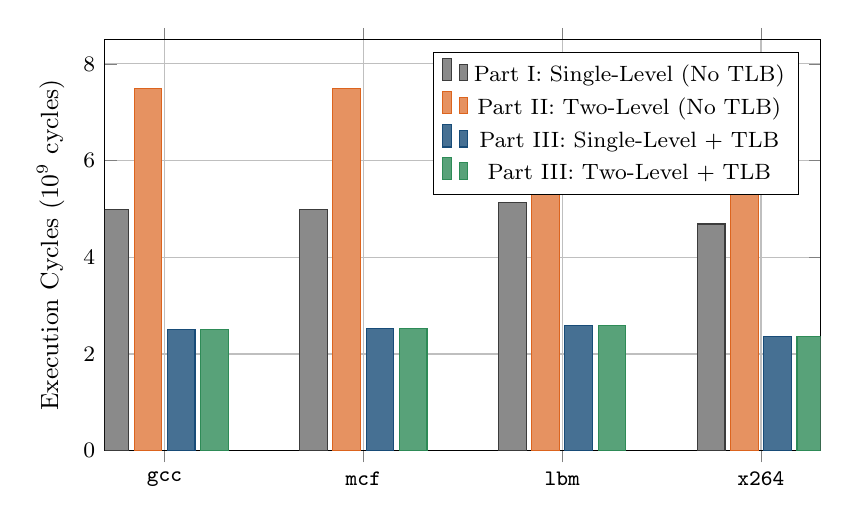
\begin{tikzpicture}
\begin{axis}[
    ybar,
    bar width=10pt,
    width=0.88\textwidth,
    height=6.8cm,
    ylabel={Execution Cycles ($10^9$ cycles)},
    symbolic x coords={\texttt{gcc}, \texttt{mcf}, \texttt{lbm}, \texttt{x264}},
    xtick=data,
    ymin=0, ymax=8.5,
    legend pos=north east,
    legend style={font=\footnotesize},
    tick label style={font=\footnotesize},
    label style={font=\small},
    grid=major
]
    \addplot[fill=darkgray!60, draw=darkgray] coordinates {
        (\texttt{gcc}, 4.989)
        (\texttt{mcf}, 4.990)
        (\texttt{lbm}, 5.137)
        (\texttt{x264}, 4.689)
    };
    \addlegendentry{Part I: Single-Level (No TLB)}

    \addplot[fill=accentorange!70, draw=accentorange] coordinates {
        (\texttt{gcc}, 7.484)
        (\texttt{mcf}, 7.485)
        (\texttt{lbm}, 7.706)
        (\texttt{x264}, 7.033)
    };
    \addlegendentry{Part II: Two-Level (No TLB)}

    \addplot[fill=primaryblue!80, draw=primaryblue] coordinates {
        (\texttt{gcc}, 2.510)
        (\texttt{mcf}, 2.521)
        (\texttt{lbm}, 2.582)
        (\texttt{x264}, 2.357)
    };
    \addlegendentry{Part III: Single-Level + TLB}

    \addplot[fill=accentgreen!80, draw=accentgreen] coordinates {
        (\texttt{gcc}, 2.513)
        (\texttt{mcf}, 2.535)
        (\texttt{lbm}, 2.583)
        (\texttt{x264}, 2.358)
    };
    \addlegendentry{Part III: Two-Level + TLB}
\end{axis}
\end{tikzpicture}
\caption{Execution cycle reduction enabled by the 128-entry TLB. The TLB cuts execution cycles by 49.7\%--66.4\% and renders the performance difference between single-level and two-level tables completely negligible.}
\label{fig:cycles_tlb_impact}
\end{figure}

\subsection{Architectural Synthesis: Neutralizing Hierarchical Latency}
The empirical results reveal two fundamental insights:
\begin{enumerate}
    \item \textbf{Massive Performance Gain}: Integrating a small 128-entry TLB delivers near-perfect hit rates ($\ge 99.4\%$). This slashes overall memory virtualization latency by \textbf{49.7\%} compared to single-level tables (from $\approx 5.0\text{B}$ to $2.5\text{B}$ cycles) and by \textbf{66.4\%} compared to two-level tables (from $\approx 7.5\text{B}$ to $2.5\text{B}$ cycles).
    \item \textbf{The Elimination of Multi-Level Penalty}: Notice in Table~\ref{tab:part3_results} and Figure~\ref{fig:cycles_tlb_impact} that the cycle count for Single-Level + TLB and Two-Level + TLB are virtually identical:
    \begin{equation}
        \Delta_{\text{Cycles}} = N_{\text{misses}} \times (601 - 401) = 200 \times N_{\text{misses}}
    \end{equation}
    In \texttt{gcc}, this difference is only $14,047 \times 200 = 2,809,400$ cycles ($< 0.11\%$ of total runtime). Because more than 99.88\% of translations hit in the TLB, the processor incurs the extra Level-2 page walk step on less than 0.12\% of instructions. \textbf{The TLB allows system architects to reap the massive 93\%+ space savings of multi-level page tables with essentially zero runtime latency penalty.}

\end{enumerate}

% =========================================================================
% SECTION 6: PART IV --- LIMITED PHYSICAL MEMORY & LRU PAGE REPLACEMENT
% =========================================================================
\section{Part IV: Limited Physical Memory \& LRU Page Replacement}

\subsection{Demand Paging Mechanics \& Latency Model}
In realistic operating environments, physical memory is substantially smaller than the virtual address space. In Part IV, physical frames are constrained:
\begin{equation}
    \text{Max Frames} = \lfloor 2^{20} \times \text{Memory Ratio} \rfloor
\end{equation}
The simulator models demand paging under an exact Least Recently Used (LRU) policy using an inverted frame table coupled with a recency list:
\begin{itemize}
    \item When an unmapped page is referenced and free frames remain, it is mapped without penalty (first page touches are free as specified).
    \item When physical memory is exhausted, a \textbf{Page Fault} occurs. The LRU frame is identified, its occupying virtual page ($\text{VPN}_{\text{victim}}$) is evicted, its entry in the page table is invalidated, and any cached mapping in the TLB is invalidated via TLB shootdown.
    \item Servicing a page fault requires disk swap access, penalizing execution by \textbf{20,000,000 cycles}.
\end{itemize}

\subsection{Thrashing Dynamics \& Page Fault Sensitivity}
Table~\ref{tab:part4_results} records the behavior of the \texttt{gcc} benchmark (working set footprint: 990 unique pages) under various physical memory constraints.

\begin{table}[h]
\centering
\caption{Part IV Results: Memory Constriction, Page Faults, and Execution Slowdown on \texttt{gcc}}
\label{tab:part4_results}
\resizebox{\textwidth}{!}{%
\begin{tabular}{lrrrrr}
\toprule
\textbf{Memory Ratio} & \textbf{Physical Frames} & \textbf{Page Faults} & \textbf{Fault Rate (\%)} & \textbf{Execution Cycles} & \textbf{Slowdown} \\
\midrule
$0.50$ (2 GB) & 524,288 & 0 & 0.000000\% & 2,509,943,906 & $1.00\times$ \\
$0.25$ (1 GB) & 262,144 & 0 & 0.000000\% & 2,509,943,906 & $1.00\times$ \\
$0.0005$ ($\approx 2.1$ MB) & 524 & 1,634 & 0.013100\% & 35,189,943,906 & \textbf{14.02$\times$} \\
$0.0002$ ($\approx 856$ KB) & 209 & 6,693 & 0.053659\% & 136,369,943,906 & \textbf{54.33$\times$} \\
\bottomrule
\end{tabular}%
}
\end{table}

\begin{figure}[h]
\centering
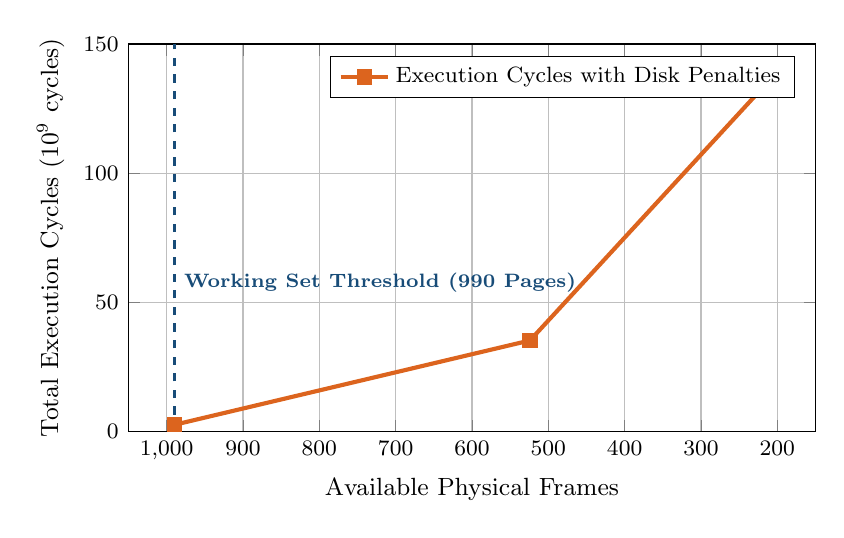
\begin{tikzpicture}
\begin{axis}[
    width=0.85\textwidth,
    height=6.5cm,
    xlabel={Available Physical Frames},
    ylabel={Total Execution Cycles ($10^9$ cycles)},
    x dir=reverse,
    grid=both,
    xmin=150, xmax=1050,
    ymin=0, ymax=150,
    legend pos=north east,
    legend style={font=\footnotesize},
    tick label style={font=\footnotesize},
    label style={font=\small}
]
    \addplot[color=accentorange, mark=square*, line width=1.5pt] coordinates {
        (990, 2.51)
        (524, 35.19)
        (209, 136.37)
    };
    \addlegendentry{Execution Cycles with Disk Penalties}

    \draw[primaryblue, dashed, line width=1.0pt] (axis cs:990,0) -- (axis cs:990,150);
    \node[anchor=south west, font=\scriptsize, text=primaryblue] at (axis cs:990,50) {\textbf{Working Set Threshold (990 Pages)}};
\end{axis}
\end{tikzpicture}
\caption{The onset of thrashing as physical frame allocation falls below the process working set. A modest 0.05\% page fault rate increases total runtime by over 54$\times$.}
\label{fig:thrashing_curve}
\end{figure}

\noindent\textbf{Critical Analysis of Paging Latency:}
Because disk access latency ($2 \times 10^7$ cycles) is five orders of magnitude slower than DRAM ($200$ cycles), even microscopic page fault rates dominate total execution time:
\begin{itemize}
    \item When physical memory exceeds 990 frames (ratios $\ge 0.001$), all active pages fit in memory, resulting in \textbf{zero page faults} and baseline latency ($2.51\text{B}$ cycles).
    \item When frames are reduced to 524 (holding $\approx 53\%$ of the active pages), the fault rate is just $0.013\%$, yet execution cycles explode to \textbf{35.19 Billion cycles ($14\times$ slowdown)}.
    \item When frames drop to 209 ($\approx 21\%$ of working set), the fault rate rises to $0.054\%$, driving execution cycles to \textbf{136.37 Billion cycles ($54.33\times$ slowdown)}.
\end{itemize}
This stark cliff illustrates the classic operating system phenomenon of \textbf{thrashing}: the system spends orders of magnitude more time stalling on I/O swaps than executing instructions.

% =========================================================================
% SECTION 7: PART V --- SIMULATOR PERFORMANCE & HIGH-SPEED OPTIMIZATION
% =========================================================================
\section{Part V: Simulator Performance \& High-Speed Optimization}

Part V evaluates the wall-clock execution speed and computational throughput of the simulator across the benchmarks.

\subsection{Optimization Strategies Implemented}
To process trace files containing tens of millions of records within seconds, we incorporated several software optimizations:
\begin{enumerate}
    \item \textbf{Bitwise Address Decomposition}: Rather than costly modulo and division operations, all VPN, offset, Level-1, and Level-2 extractions use single-cycle bitwise shifts and bitmasks:
    \begin{lstlisting}[language=C++]
uint32_t get_vpn() const { return address >> 12; }
uint32_t get_l1_index() const { return (address >> 22) & 0x03FF; }
uint32_t get_l2_index() const { return (address >> 12) & 0x03FF; }
    \end{lstlisting}
    \item \textbf{$O(1)$ TLB LRU Maintenance via Splice}: Rather than linearly searching an array or shifting vector elements upon every hit, the TLB uses \texttt{std::list::splice} on list iterators held in \texttt{std::unordered\_map}:
    \begin{lstlisting}[language=C++]
bool TLB::lookup(uint32_t vpn, uint32_t& frame_out) {
    auto it = tlb_map.find(vpn);
    if (it != tlb_map.end()) {
        frame_out = it->second->frame;
        lru_list.splice(lru_list.begin(), lru_list, it->second); // O(1) move to MRU
        return true;
    }
    return false;
}
    \end{lstlisting}
    \item \textbf{Zero Heap Allocations on the Critical Path}: Once inner tables or TLB nodes are allocated, lookups, bit modifications, and hash updates require zero dynamic memory allocation (\texttt{new}/\texttt{malloc}).
    \item \textbf{Optimized Compiler Toolchain}: Compiled with \texttt{-O2} optimization flags, enabling aggressive function inlining and loop vectorization.
\end{enumerate}

\subsection{Wall-Clock Execution Benchmark Profile}
Table~\ref{tab:part5_timing} summarizes the execution time and throughput on an x86-64 host machine.

\begin{table}[h]
\centering
\caption{Part V Simulator Wall-Clock Performance and Throughput}
\label{tab:part5_timing}
\resizebox{\textwidth}{!}{%
\begin{tabular}{lrrr}
\toprule
\textbf{Benchmark Trace} & \textbf{Total Trace Entries} & \textbf{Wall-Clock Time (s)} & \textbf{Throughput (Million Accesses/s)} \\
\midrule
\texttt{gcc} & 12,473,306 & 2.51 s & \textbf{4.97 M accesses/s} \\
\texttt{mcf} & 12,474,523 & 2.86 s & \textbf{4.36 M accesses/s} \\
\texttt{lbm} & 12,843,431 & 2.77 s & \textbf{4.63 M accesses/s} \\
\texttt{x264} & 11,721,344 & 2.28 s & \textbf{5.14 M accesses/s} \\
\bottomrule
\end{tabular}%
}
\end{table}

The simulator consistently achieves processing throughputs between \textbf{4.36 and 5.14 million memory accesses per second}, enabling multi-million-access trace files to be simulated in under three seconds.

% =========================================================================
% SECTION 8: CONCLUSIONS & ARCHITECTURAL SUMMARY
% =========================================================================
\section{Conclusions \& Architectural Insights}

This comprehensive laboratory investigation yields five overarching architectural conclusions:
\begin{enumerate}
    \item \textbf{The Inefficiency of Flat Page Tables}: A linear single-level page table requires contiguous kernel memory for the entire address space ($1,048,576$ entries), yet typical benchmarks utilize fewer than $2,200$ pages. This results in an abysmal page table utilization of $< 0.2\%$, making flat page tables impractical for 32-bit and 64-bit systems.
    \item \textbf{The Superiority of Hierarchical Multi-Level Tables}: Two-level hierarchical page tables with on-demand allocation reduce page table memory overhead by \textbf{93.07\% to 99.32\%}, enabling systems to support numerous processes concurrently without exhausting physical memory.
    \item \textbf{The Synergistic Role of the TLB}: While multi-level page tables introduce extra memory lookup steps (400 vs.\ 200 cycles for page walks), a small 128-entry fully associative TLB achieves hit rates exceeding \textbf{99.4\% to 99.9\%}. This virtually eliminates the hierarchical walk penalty, yielding the optimal architectural balance: minimal memory overhead with single-cycle translation speed.
    \item \textbf{Validation of Pareto Locality (Hypothesis B)}: Access distributions across virtual pages strictly follow a Pareto distribution, with the top 10\% of pages capturing over 82\% of memory references. This concentrated working set explains why a compact 128-entry TLB delivers such high hit rates.
    \item \textbf{The Severe Cost of Thrashing}: When physical frame allocations drop below a process's active working set, disk fault penalties ($20,000,000$ cycles) trigger exponential execution slowdowns (over $54\times$ degradation), demonstrating the critical importance of effective working-set management in operating system schedulers.
\end{enumerate}

\end{document}
